\begin{frame}
    \frametitle{Phép cộng vector}
    \begin{columns}
    \begin{column}{0.5\textwidth}
        Để xác định vị trí của viên đá, thay vì xác định trực tiếp, ta sẽ để Hirrus xác định vị trí của viên đá, rồi ta sẽ xác định vị trí của Hirrus.
        \begin{figure}
            \centering
            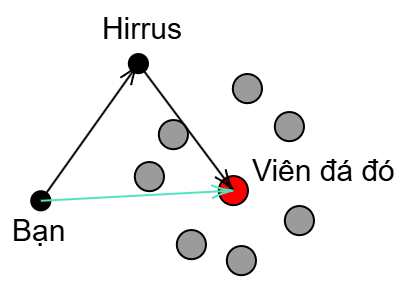
\includegraphics[width=0.7\textwidth]{Slides/Figure/HirrusAndStones.png}
        \end{figure}
    \end{column}
    \begin{column}{0.5\textwidth}
        \(\longrightarrow\) \textbf{Phép cộng vector}:
        \begin{figure}[H]
            \centering
            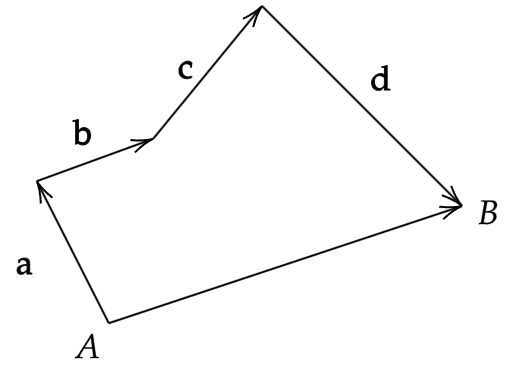
\includegraphics[width=0.7\textwidth]{Slides/Figure/congvector.png}
            \caption{$\mathbf{a}+\mathbf{b}+\mathbf{c}+\mathbf{d}=\mathbf{AB}$}
        \end{figure}
        Về tổng quát, \(|\mathbf a +\mathbf b| \neq a+b\).
        \end{column}
    \end{columns}
\end{frame}

\begin{frame}
\frametitle{Hai phép nhân vector}
\begin{columns}
\begin{column}{0.5\textwidth}
    \textbf{Phép nhân vô hướng hai vector}
    \begin{figure}
    \centering
    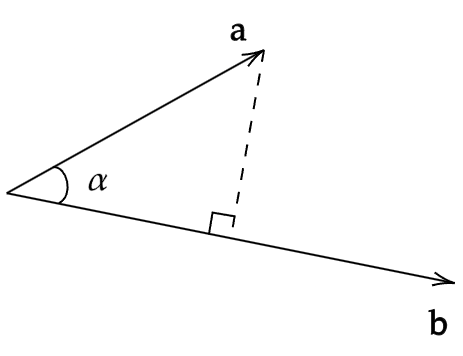
\includegraphics[width=0.65\textwidth]{Slides/Figure/tichcham.png}
    \end{figure}
    \begin{itemize}
        \item Kết quả là một số vô hướng.
        \item \(\mathbf a \cdot \mathbf b = ab \cos \alpha\)
    \end{itemize}
\end{column}
\begin{column}{0.5\textwidth}
    \textbf{Phép nhân có hướng hai vector}
    \begin{figure}
    \centering
    
\includegraphics[width=0.5\textwidth]{Slides/Figure/tichcheo.png}
    \end{figure}
    \begin{itemize}
        \item Kết quả là một vector.
        \item \(|\mathbf a \times \mathbf b| = ab \sin \alpha\)
    \end{itemize}
\end{column}
\end{columns}
\end{frame}